\section{Introduction}
\label{s:intro}

%\wajih{I have updated the macro logs as it does not make sense to use \ logs for just "system". I have changed the macro to "system logs". Make sure the paper is consistent with that.}

% The effectiveness of IDSes hinges on their ability to accurately detect these threats, maintain low false positive rates, and operate with minimal resource consumption, ensuring system performance is not compromised.

%\wajih{Give the workflow of MSSP and cite that organizations outsource their security. If you find any numbers on how many comapnies use MSSP and outsource their security operations that would be great. If you find any realworld attack examples on MSSP where the data was leaked that would be great as well. }

Intrusion Detection Systems (\ids) are crucial for countering Advanced Persistent Threats (APTs) in enterprises, as evidenced by major attacks, such as Solar Winds~\cite{solarwinds} and NotPetya~\cite{notpetya}. Given their stealth and persistence, many enterprises rely on Managed Security Service Providers (MSSPs) to improve their defenses. A survey~\cite{msspsurvey} involving over 5,000 IT professionals reported that about 75\% of companies use MSSPs. These providers integrate their security systems with clients' systems to manage \logs, typically configuring the clients' systems to transmit \logs to the cloud for analysis. Figure~\ref{mssp} illustrates this MSSP operational architecture.


Recently, Provenance-based IDS (PIDS)~\cite{streamspot,provdetector2020,wang2022threatrace,shadewatcher,yangprographer,han2020unicorn} have emerged as a highly effective means of enhancing intrusion detection. These systems leverage the extensive contextual information provided by \logs to bolster their detection capabilities. PIDS operate by converting \logs into provenance graphs, which are then analyzed using machine learning techniques, such as Graph Neural Networks (\gnnshort), to identify and learn patterns of benign activity. By continuously monitoring these patterns, PIDS can detect deviations that may indicate potential security threats. Upon detecting such anomalous graph patterns, the PIDS generate alerts to prompt further investigation.


Despite PIDS potential, the current operational mode of MSSPs and the state-of-the-art techniques for intrusion detection face significant challenges in the complex landscape of enterprise security. Table~\ref{tab:limitations} provides an overview of the limitations of the existing systems, with further discussion below.



%\wajih{Please put the MSSP figure we talk about here.}



%\wajih{please use consistent font size which means only two sizes one of headings and one for the body. Could you show that logs go to centralized storage. Also, we talked that we will say "Plain-Text Audit Logs" instead of "Logs". You need to start taking notes while we are discussing things.}



\smallskip
\noindent
\textbf{C1: Lack of Privacy Preservation:} The current operational mode of MSSPs and PIDS involves a centralized infrastructure that requires client machines to transmit their \logs to a central server. Notable state-of-the-art systems, such as \flash\cite{flash2024} and \kairos~\cite{cheng2023kairos} function under the assumption that \logs from various machines will be available at a centralized location for processing. This central aggregation of data is essential, as \pids employ advanced deep learning techniques to model and understand benign behaviors effectively. These models necessitate large datasets to learn normal system behaviors accurately, and data from a single user's machine proves to be inadequate. Our experiments with \flash, which was trained using data from just a single host in the DARPA OPTC dataset~\cite{darpaoptc}, exhibited a significant performance drop -- a 40\% decrease in the F-score -- when compared to training with multi-host data. However, this centralized approach to data handling introduces substantial privacy risks. \logs contain detailed records of system activities, potentially including sensitive data, such as specific URLs visited, IP addresses, and user application usage. These privacy issues are not merely theoretical; they have been highlighted in a recent report by Datadog~\cite{datadog}, a leading provider of system monitoring services. Note that existing decentralized IDS, such as DistDet \cite{dong2023distdet}, employ the use of a Hierarchical System Event Tree (HST) for storing all system event attributes. However, these HSTs are transmitted in plaintext to the server, breaching user log privacy.
%\wajih{fix this last sentence. make sure that it is technically correct. the goal is to say that disdet has privacy problems.}

\begin{figure}[t!]
    \centering
    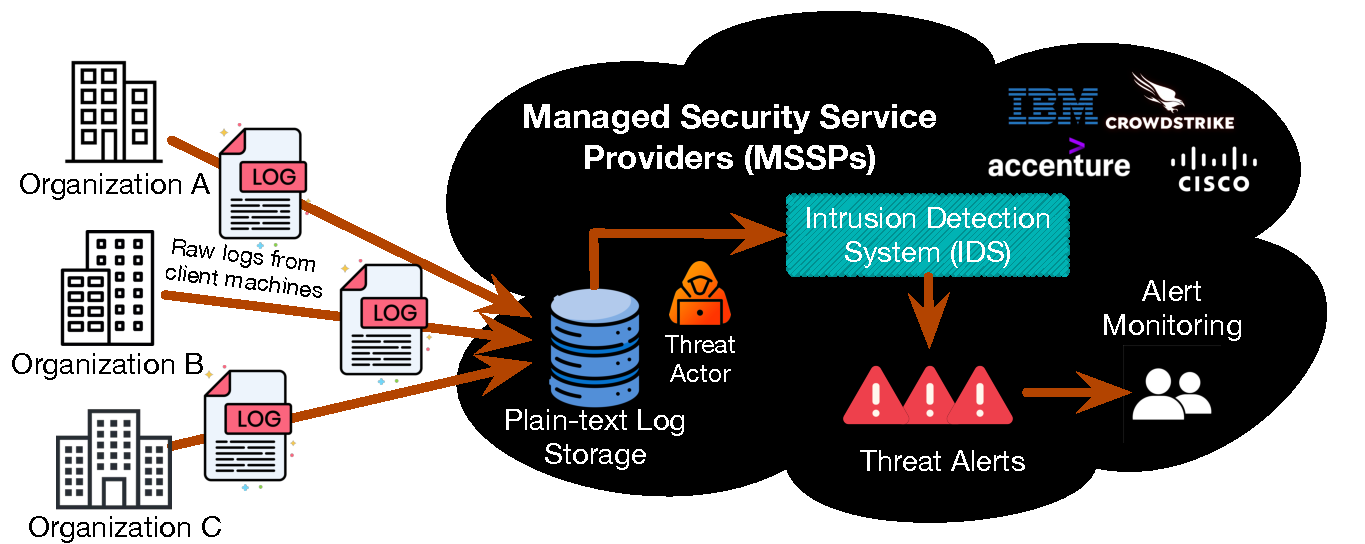
\includegraphics[width=0.45\textwidth]{fig/mssp.pdf}
    \caption{The MSSP architecture for intrusion detection. The plain-text system logs are first collected in a centralized storage managed by the MSSP. Then these system logs are analyzed for threats.}
    \label{mssp}
    \vspace{-4ex}
  \end{figure}
    
\smallskip
\noindent
\textbf{C2: Excessive Network Overhead:} In the context of MSSPs and centralized PIDS, the requirement to transmit \logs over the network for threat detection can result in substantial network overhead. Modern systems often generate logs amounting to gigabytes per day, imposing significant network costs on both users and organizations~\cite{inam2023sok,hossain+depend}. Our analysis of systems, such as \flash and \kairos, using the \optc dataset as detailed in Section~\ref{cost_metric}, highlights this issue. For an organization of a similar scale to that represented in the \optc dataset, with an equivalent number of hosts, the daily volume of logs transmitted could easily reach 1000 GB. This immense volume of data not only incurs considerable network expenses daily but also presents a significant challenge for users with limited network bandwidth, who may struggle to upload such large amounts of data efficiently. Note that \disdet reduces network costs by summarizing system events in hierarchical tree data structures but compromises privacy because HSTs must be sent to the server in plain text. Additionally, \disdet identifies anomalies as events simply missing from the benign HST, a method prone to false alarms in dynamically changing system environments.

%\wajih{is it possible to say something about DistDet here? I am worried that the reviewers are just going to say that you are building an extension of DisDet}

\smallskip
\noindent
\textbf{C3: Limited Scalability:} The centralized approach employed by current PIDS poses scalability challenges as the number of hosts within an organization grows. Such centralization serves as a bottleneck, leading to log congestion and thereby impeding efficient intrusion detection at scale. Additionally, for large organizations, the centralized accumulation of logs can lead to significant disk storage overhead. To accommodate an increasing number of hosts, organizations must continually allocate more resources. Consequently, the existing approach to threat detection lacks inherent scalability. Our evaluations of \flash and \kairos demonstrate that these systems would face log congestion in organizations of a size comparable to that represented by the \optc dataset. As detailed in Section~\ref{sec:eval}, \flash would require 27.7 hours, and \kairos 56.6 hours, to process a single day's worth of logs from the \optc dataset.

    
    %\wajih{Again you need to add more details here about scalability issues. Having specific numbers for existing PIDS is important. Also cite those existing PIDS }


%\wajih{I added C1, C2, C3 with each challenge above. You need to refer to each of the challenge below and tell how you solve that challenge. Something like: "To address C1, we do blah blah"}

To address these challenges, we introduce \Sys, a novel privacy-preserving PIDS that integrates provenance graph representation learning with Federated Learning (FL). In \Sys, client logs remain local, which significantly enhances user privacy by ensuring sensitive data does not leave the client's environment (C1). Each client independently trains \gnnshort models, and these models are aggregated on a central server with those from other clients, capturing diverse activity patterns across organizations without transmitting actual logs, thus minimizing network overhead. Instead, the only data transmitted are model updates, which are mere kilobytes per client, significantly reducing the network burden (C2). All major computations, including the training and operational phases of \Sys, take place locally on client machines, using their computing resources to process provenance graphs derived from their logs for real-time threat detection. This approach allows \Sys to scale effectively with the addition of more hosts, each utilizing its own computing power and storage, addressing scalability and efficiency comprehensively (C3).


\begin{table}[t!]
  \centering
  \scriptsize
    %\caption{Limitations of existing PIDS. \wajih{Add in caption that which PIDS are not specified in the table and why.}}
    \caption{Existing PIDS limitations: \flash and \kairos outperform other existing PIDS systems ~\cite{wang2022threatrace,han2020unicorn,streamspot,yangprographer,shadewatcher,provdetector2020}. Therefore, we have excluded these PIDSes from the table. }
    \setlength{\tabcolsep}{10pt}
      \begin{tabular}{ | c | c | c | c |}

        \hline
             & \bf Data & \bf Network  & \bf Scalability \\
             & \bf  Privacy & \bf  Overhead &  \\
        \hline
        \hline
        \disdet~\cite{dong2023distdet} & NO                       & LOW      & HIGH       \\
        \hline
        \flash~\cite{flash2024}     & NO            & HIGH             & MEDIUM      \\
        \hline
        \kairos~\cite{cheng2023kairos}     & NO            & HIGH             & LOW         \\
        \hline
        {\bf\Sys}  & YES                & LOW               & HIGH        \\
        \hline
      \end{tabular}
      \label{tab:limitations}
  \end{table}


\subsection{Our Approach and Main Contributions}

The implementation of FL for a privacy-preserving PIDS introduces multiple challenges. Firstly, model aggregation in a federated setting becomes complex due to heterogeneous data distributions from clients running different applications, leading to suboptimal unified model performance. Additionally, data imbalances across clients, where smaller data contributors have less impact on the federated model, skew the learning outcomes. Another significant hurdle is the inconsistent semantic information produced by independently trained \wordvec models on different client machines. This inconsistency across semantic encoders complicates the effectiveness of the global models, resulting in inaccurate system behavior representations due to varied feature vector qualities.



To effectively address the challenges of heterogeneity and data imbalance, we have designed a novel ensemble learning framework. In this framework, each submodel is trained to specialize in learning system activities associated with specific process entities, which are standardized across all clients. This standardization is facilitated by a sophisticated categorization scheme enabled by our dual-server architecture. Through this system, process entities from all clients are organized into \textit{K} privacy-preserving bins. Each client then aligns its process nodes with these bins, constructs a provenance subgraph for each bin, and trains a \gnnshort model on these graphs. The models from all clients are then aggregated into \textit{K} model pairs, forming a comprehensive global ensemble model set. This strategic approach ensures that models with similar data distributions are merged effectively, thereby maintaining the integrity of unique activity patterns across diverse client environments.

To address semantic inconsistencies in \wordvec models, we implement a \wordvec harmonization scheme utilizing a dual-server architecture. In this setup, a central server issues encryption keys to clients, allowing them to securely encode \wordvec tokens. Subsequently, a utility server processes these encrypted tokens to achieve a unified, privacy-preserving vector representation. This method ensures that sensitive data remains protected while facilitating accurate and consistent semantic encoding across different clients.


%\wajih{Add one paragraph how you solve that above mentioned challenge. This will highlight the novelty of your system.}

%\wajih{make sure to say two or three lines about adversarial attacks and say that more details are present in the discussion section.}

%\wajih{Add one paragraph related to evaluation results.}

We have conducted extensive evaluations of our system's effectiveness using open-source datasets from \darpa, specifically E3~\cite{error3}, E5~\cite{bug5}, and \optc~\cite{anjum2021analyzing}. These datasets encompass a broad spectrum of attack scenarios and system behaviors. Our findings indicate that \Sys achieves high detection performance, with an average precision of 96\% and recall of 97\%. Thus, our system performs comparably to state-of-the-art centralized systems like \flash and \kairos. As detailed in section~\ref{cost_metric}, our system achieves a 170-fold reduction in communication and storage costs compared to \flash and \kairos. Since our technique is decentralized, our inference time is bounded by the client with the most log data; it will only take approximately 3 minutes to run inference on the complete \optc dataset, whereas \flash and \kairos take many hours. Employing FL exposes our system to certain types of adversarial attacks, such as model poisoning, inference, and gradient attacks. We provide a comprehensive analysis of our system's resilience against these attacks in Section~\ref{sec:discussion}. We also present a detailed analysis of the privacy protection of our system in Section~\ref{privacy}.

%\wajih{Add list of main contributions}
The main contributions of our work are as follows:

\begin{itemize}[topsep=.1ex,itemsep=-.1ex,leftmargin=*]
    \item[--] To the best of our knowledge, we are the first to introduce federated provenance graph learning in the domain of IDS with our system, \Sys.
    \item[--] We have introduced a novel \textbf{ensemble learning} and \textbf{process entity categorization} framework for dealing with diverse heterogeneous client data distributions.
    \item[--] We developed a sophisticated \textbf{\wordvec harmonization framework} using a multi-server architecture for secure private aggregation of semantic attributes.
    \item[--] We conduct a comprehensive evaluation of our technique on real-world datasets, demonstrating \Sys's effectiveness in detecting system threats while being scalable and privacy-preserving.
\end{itemize}

\PP{Availability.} \wajih{Add a link for your code here.}